\documentclass[12pt, letterpaper]{article}
\usepackage[english]{babel} % Sets the language and regional settings for English documents
\usepackage[utf8]{inputenc} % Allows the use of UTF-8 characters in the document
\usepackage[T1]{fontenc} % Specifies t\subsubsection*{Forma canónica reducida}
\usepackage[margin=2cm]{geometry} % Sets the page margins
\usepackage{makeidx} % Enables the creation of indexes
% \usepackage{natbib} % Provides flexible bibliography support
\usepackage{url} % Allows the use of URLs
\usepackage{enumitem} % Customizes the appearance of lists
\usepackage{listings} % Provides syntax highlighting for code listings
\usepackage[dvipsnames]{xcolor} % Allows the use of colors
\usepackage{parskip} % Modifies paragraph spacing
\usepackage{graphicx} % Enables the inclusion of graphics
\usepackage{tikz} % Allows the creation of graphics and diagrams
\usepackage{float}
\usepackage{hyperref} % Enables the creation of hyperlinks
\usepackage{amsmath} % Provides additional math environments and commands
\usepackage{circuitikz} % Allows the creation of electrical circuits
\usepackage{adjustbox} % Adjusts the size of the circuit diagrams
\usepackage{tcolorbox}
\usepackage{diagbox} % Allows the use of diagonal boxes in table cells
\usepackage{colortbl} % Allows coloring of table cells
\hypersetup{
    colorlinks=true,
    linkcolor=blue,
    urlcolor=blue
}
\usepackage{breakurl} % permite que los links se rompan en varias líneas
\definecolor{mygray}{gray}{0.9}

\usetikzlibrary{shapes.geometric, positioning}

\lstset{
	language=SQL,
	basicstyle=\ttfamily\small,
	keywordstyle=\color{blue},
	commentstyle=\color[rgb]{0,0.5,0},
	stringstyle=\color{red},
	numbers=left,
	numberstyle=\tiny\color{gray},
	stepnumber=1,
	numbersep=10pt,
	backgroundcolor=\color{white},
	showspaces=false,
	showstringspaces=false,
	breaklines=true,
	frame=single,
	tabsize=2, captionpos=b, lineskip=-1pt,
	extendedchars=true,
	literate={á}{{\'a}}1 {é}{{\'e}}1 {í}{{\'i}}1 {ó}{{\'o}}1 {ú}{{\'u}}1 {Á}{{\'A}}1 {É}{{\'E}}1 {Í}{{\'I}}1 {Ó}{{\'O}}1 {Ú}{{\'U}}1 {ñ}{{\~n}}1 {Ñ}{{\~N}}1 {¿}{{\textquestiondown}}1 {¡}{{\textexclamdown}}1
}

% VHDL language configuration
\lstdefinelanguage{VHDL}{
	morekeywords={entity, architecture, signal, port, in, out, inout, begin, end, process, if, then, else, elsif, case, when, others, for, while, loop, wait, library, use, std_logic, std_logic_vector, integer, boolean, rising_edge, falling_edge, component, generic, map, downto, to, and, or, not, xor, nand, nor, xnor},
	morecomment=[l]{--},
	morestring=[b]",
	sensitive=false,
	alsoletter={_}
}

% VHDL listings style
\lstdefinestyle{vhdl}{
	language=VHDL,
	basicstyle=\ttfamily\small,
	keywordstyle=\color{blue}\bfseries,
	commentstyle=\color[rgb]{0,0.6,0}\itshape,
	stringstyle=\color{red},
	numbers=left,
	numberstyle=\tiny\color{gray},
	stepnumber=1,
	numbersep=10pt,
	backgroundcolor=\color{white},
	showspaces=false,
	showstringspaces=false,
	breaklines=true,
	frame=single,
	tabsize=2,
	captionpos=b,
	lineskip=-1pt,
	extendedchars=true
}

\graphicspath{ {./img/} } % Sets the path for the graphics

\newlist{biblio}{enumerate}{1}
\setlist[biblio,1]{label=[\arabic*]}

\makeindex

\begin{document}

\begin{titlepage}

	\begin{tikzpicture}[remember picture,overlay]
		\node[anchor=north west, inner sep=30] at (current page.north west) {
			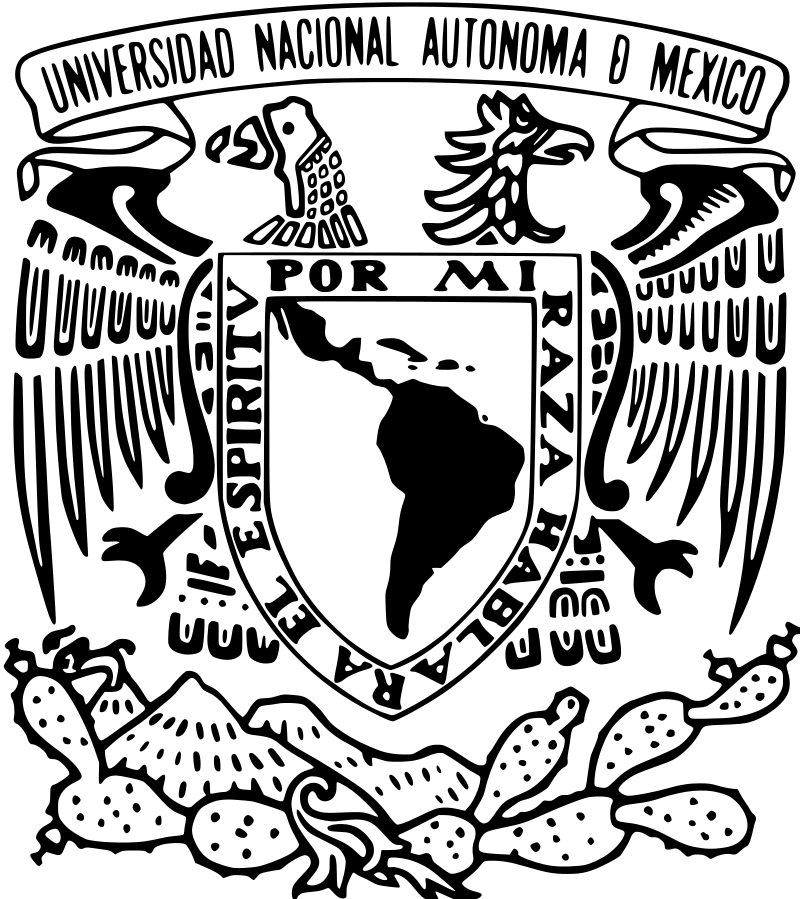
\includegraphics[width=4cm]{escudoUNAM.png}
		};

		\node[anchor=north east, inner sep=30] at (current page.north east) {
			
\includegraphics[width=4cm]{escudoFI.png}
		};
	\end{tikzpicture}

	\begin{center}
		\vspace*{3cm}

		\Huge
		\textbf{Previo 4 - Escalamiento de Impedancia y Frecuencia}\\

		\vspace{2.5cm}

		\Huge
		\textbf{Facultad de Ingeniería}\\
		Circuitos Electrónicos\\
		\textbf{Ing. Martha Isela Torres Hernández} \\
		2026-1\\

		\vspace{2.5cm}

		\textbf{Grupo:} 4\\

		\vspace{2.5cm}

		\Huge
        \textbf{Integrantes Brigada 6:}\\
		Ugartechea González Luis Antonio\\
		Tepal Briseño Hansel Yael\\
		\textbf{Fecha de entrega:} 28 de octubre del 2025\\
		\vspace{2.5cm}
	\end{center}
\end{titlepage}

\section{Escalamiento de Impedancia}

El \textbf{escalamiento de impedancia} (o escalamiento de magnitud) es un proceso que cambia el nivel de impedancia de todos uno o varios componentes de un circuito por otro valor, \textbf{sin modificar la función de transferencia} del circuito.

Esto significa que características como la frecuencia de corte, la frecuencia de resonancia, el ancho de banda y la ganancia (en el caso de amplificadores operacionales) permanecen exactamente iguales.

Se utiliza un factor de escalamiento de magnitud, denotado como \(k_m\).

\subsection*{Fórmulas de Escalamiento de Impedancia}

En el escalamiento de impedancia se usa un valor \(k_m\), este valor nos sirve para escalar los valores de los componentes del circuito de acuerdo a los requerimeintos del problema, de igual forma podemos obtener el valor de \(k_m\) si conocemos los valores iniciales y finales de un componente. Estas fórmulas son las siguientes:

\begin{itemize}
    \item \textbf{Resistores:} La impedancia de un resistor es \(Z_R = R\). Para escalarla por \(k_m\), el nuevo valor \(R_o\) debe ser:

    \[k_m = \frac{R_o}{R} \]
    \[ R_o = k_m \cdot R \]

    \textbf{Donde:}
    \begin{itemize}
        \item \(R_o\): Valor del resistor objetivo.
        \item \(R\): Valor del resistor inicial.
    \end{itemize}

    \item \textbf{Inductores:} La impedancia de un inductor es \(Z_L = sL\). Para escalar esto por \(k_m\), necesitamos \(Z_{L_o} = k_m (sL) = s (k_mL)\). Por lo tanto, la nueva inductancia \(L_o\) es:

    \[k_m = \frac{L_o}{L} \]
    \[ L_o = k_m \cdot L \]

    \textbf{Donde:}
    \begin{itemize}
        \item \(L_o\): Valor del inductor objetivo.
        \item \(L\): Valor del inductor inicial.
    \end{itemize}

    \item \textbf{Capacitores:} La impedancia de un capacitor es \(Z_C = \frac{1}{s C}\). Para escalarla por \(k_m\), necesitamos \(Z_{C_o} = k_m \left( \frac{1}{s C} \right) = \frac{1}{s (C k_m)}\). Por lo tanto, la nueva capacitancia \(C_o\) es:

    \[k_m = \frac{C}{C_o} \]
    \[C_o = \frac{C}{k_m} \]

    \textbf{Donde:}
    \begin{itemize}
        \item \(C_o\): Valor del capacitor objetivo.
        \item \(C\): Valor del capacitor inicial.
    \end{itemize}
\end{itemize}

\begin{tcolorbox}[colback=mygray, colframe=LimeGreen, boxrule=0.7pt, arc=2pt, boxsep=1pt, left=2pt, right=2pt, top=2pt, bottom=2pt, title=Ejemplo de Escalamiento de Impedancia]
    Dado el siguiente circuito RC en serie con \(V_i = 20 sen(2000 \pi t)\),\(R = 15 k \Omega\) y \(C = 1 \mu F\)
    \begin{figure}[H]
        \centering
        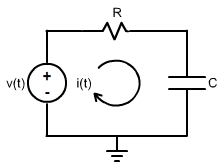
\includegraphics[width=0.3\textwidth]{rc_serie.png}
        \caption{Circuito RC en serie}
        \label{fig:rc_serie}
    \end{figure}

    Determinar el valor de los capacitor si sustituimos el resistor por \(R_o = 1 k \Omega\) usando un escalamiento de impedancia.

    \textbf{Solución:}

    Primero, calculamos el factor de escalamiento de magnitud \(k_m\):
    \[k_m = \frac{R_o}{R} = \frac{1 k \Omega}{15 k \Omega} = \frac{1}{15} \]

    Luego, usamos este valor para encontrar el nuevo valor del capacitor \(C_o\):
    \[C_o = \frac{C}{k_m} = \frac{1 \mu F}{\frac{1}{15}} = 15 \mu F \]

    Por lo tanto, el nuevo valor del capacitor es \(C_o = 15 \mu F\).
\end{tcolorbox}

\section{Escalamiento de Frecuencia}

El \textbf{escalamiento de frecuencia} es un proceso que desplaza la respuesta en frecuencia de un circuito por un factor constante, \textbf{sin modificar la función de transferencia} del circuito.

Esto tiene muchas funcionalidades, entre ellas nos sirve para manipular componentes de un circuito en base a un cambio en la frecuencia de la señal de entrada.

Se utiliza un factor de escalamiento de frecuencia, denotado como \(k_f\).

\subsection*{Fórmulas de Escalamiento de Frecuencia}

En el escalamiento de frecuencia se usa un valor \(k_f\), este valor nos sirve para escalar los valores de los componentes del circuito de acuerdo a los requerimeintos del problema, de igual forma podemos obtener el valor de \(k_f\) si conocemos el valor inicial y final de la frecuencia en la señal de entrada. Para obtener \(k_f\) se usa la siguiente fórmula:

\[k_f = \frac{{\omega t}_i}{{\omega t}_o}\]

\textbf{Donde:}

\begin{itemize}
    \item \({\omega t}_i\): Frecuencia angular inicial (\(\pi \frac{rad}{s}\)).
    \item \({\omega t}_o\): Frecuencia angular objetivo (\(rad/s\)).
\end{itemize}

A partir de este valor, se pueden escalar los componentes del circuito de la siguiente manera:

\begin{itemize}
    \item \textbf{Resistores:} La impedancia de un resistor (\(Z_R = R\)) no depende de la frecuencia, por lo que su valor no se modifica.

    \[ R_o = R \]

    \textbf{Donde:}
    \begin{itemize}
        \item \(R_o\): Valor del resistor objetivo.
        \item \(R\): Valor del resistor inicial.
    \end{itemize}

    \item \textbf{Inductores:} La impedancia de un inductor es \(Z_L = sL\). Para escalar la frecuencia por \(k_f\), la nueva inductancia \(L_o\) es:

    \[k_f = \frac{L}{L_o} \]
    \[L_o = \frac{L}{k_f} \]

    \textbf{Donde:}
    \begin{itemize}
        \item \(L_o\): Valor del inductor objetivo.
        \item \(L\): Valor del inductor inicial.
    \end{itemize}

    \item \textbf{Capacitores:} La impedancia de un capacitor es \(Z_C = \frac{1}{s C}\). Para escalar la frecuencia por \(k_f\), la nueva capacitancia \(C_o\) es:

    \[k_f = \frac{C}{C_o} \]
    \[C_o = \frac{C}{k_f} \]

    \textbf{Donde:}
    \begin{itemize}
        \item \(C_o\): Valor del capacitor objetivo.
        \item \(C\): Valor del capacitor inicial.
    \end{itemize}
\end{itemize}

\begin{tcolorbox}[colback=mygray, colframe=LimeGreen, boxrule=0.7pt, arc=2pt, boxsep=1pt, left=2pt, right=2pt, top=2pt, bottom=2pt, title=Ejemplo de Escalamiento de Frecuencia]
    Dado el siguiente circuito RC en serie con \(V_i = 20 sen(2000 \pi t)\),\(R = 15 k \Omega\) y \(C = 1 \mu F\)
    \begin{figure}[H]
        \centering
        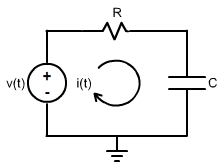
\includegraphics[width=0.3\textwidth]{rc_serie.png}
        \caption{Circuito RC en serie}
        \label{fig:rc_serie}
    \end{figure}

    Determinar el valor de los capacitor si sustituimos si la frecuencia de la señal de entrada por \(V_i = 20 sen(4000 \pi t)\) usando un escalamiento de frecuencia.

    \textbf{Solución:}

    Primero, calculamos el factor de escalamiento de frecuencia \(k_f\):
    \[k_f = \frac{\omega_i}{\omega_o} = \frac{2000 \pi}{4000 \pi} = 0.5 \]

    Luego, usamos este valor para encontrar el nuevo valor del capacitor \(C_o\):
    \[C_o = C \cdot k_f = 1 \mu F \cdot 0.5 = 0.5 \mu F \]

    Por lo tanto, el nuevo valor del capacitor es \(C_o = 0.5 \mu F\).
\end{tcolorbox}

\section{Escalamiento Combinado}

El \textbf{escalamiento combinado} es un proceso que aplica simultáneamente un escalamiento de impedancia (definido por \(k_m\)) y un escalamiento de frecuencia (definido por \(k_f\)).

Este método es el más utilizado en la práctica, ya que permite tomar un circuito "prototipo" (usualmente normalizado con \(R=1\Omega\) y \(\omega=1\) rad/s) y transformarlo directamente a los valores de impedancia y frecuencia de operación requeridos en una aplicación real.

\subsection*{Fórmulas de Escalamiento Combinado}

Para el escalamiento combinado, se deben conocer ambos factores, \(k_m\) y \(k_f\). Generalmente, \(k_m\) se determina a partir del nuevo valor deseado para los resistores [cite: 10] y \(k_f\) se determina a partir de la nueva frecuencia angular objetivo.

\[k_f = \frac{\omega_o}{\omega_i} \]

\textbf{Donde:}
\begin{itemize}
    \item \(\omega_o\): Frecuencia angular objetivo (\(\pi \frac{rad}{s}\)).
    \item \(\omega_i\): Frecuencia angular inicial (\(\pi \frac{rad}{s}\)).
\end{itemize}

A partir de este factor, los nuevos valores de los componentes se calculan de la siguiente manera:

\begin{itemize}
    \item \textbf{Resistores:} El valor del resistor solo es afectado por el escalamiento de magnitud \(k_m\)[cite: 10, 23].

    \[ R_o = k_m \cdot R \]

    \textbf{Donde:}
    \begin{itemize}
        \item \(R_o\): Valor del resistor objetivo.
        \item \(R\): Valor del resistor inicial.
    \end{itemize}

    \item \textbf{Inductores:} El valor del inductor es afectado por ambos factores.

    \[ L_o = \left( \frac{k_m}{k_f} \right) L \]

    \textbf{Donde:}
    \begin{itemize}
        \item \(L_o\): Valor del inductor objetivo.
        \item \(L\): Valor del inductor inicial.
    \end{itemize}

    \item \textbf{Capacitores:} El valor del capacitor es afectado por ambos factores.

    \[ C_o = \frac{C}{k_m k_f} \]

    \textbf{Donde:}
    \begin{itemize}
        \item \(C_o\): Valor del capacitor objetivo.
        \item \(C\): Valor del capacitor inicial.
    \end{itemize}
\end{itemize}

\begin{tcolorbox}[colback=mygray, colframe=LimeGreen, boxrule=0.7pt, arc=2pt, boxsep=1pt, left=2pt, right=2pt, top=2pt, bottom=2pt, title=Ejemplo de Escalamiento Combinado]
    Dado el siguiente circuito RLC en serie con \(V_i = 20 sen(2000 \pi t)\),\(R = 15 k \Omega\), \(L = 10 mH\) y \(C = 1 \mu F\).

    \begin{figure}[H]
        \centering
        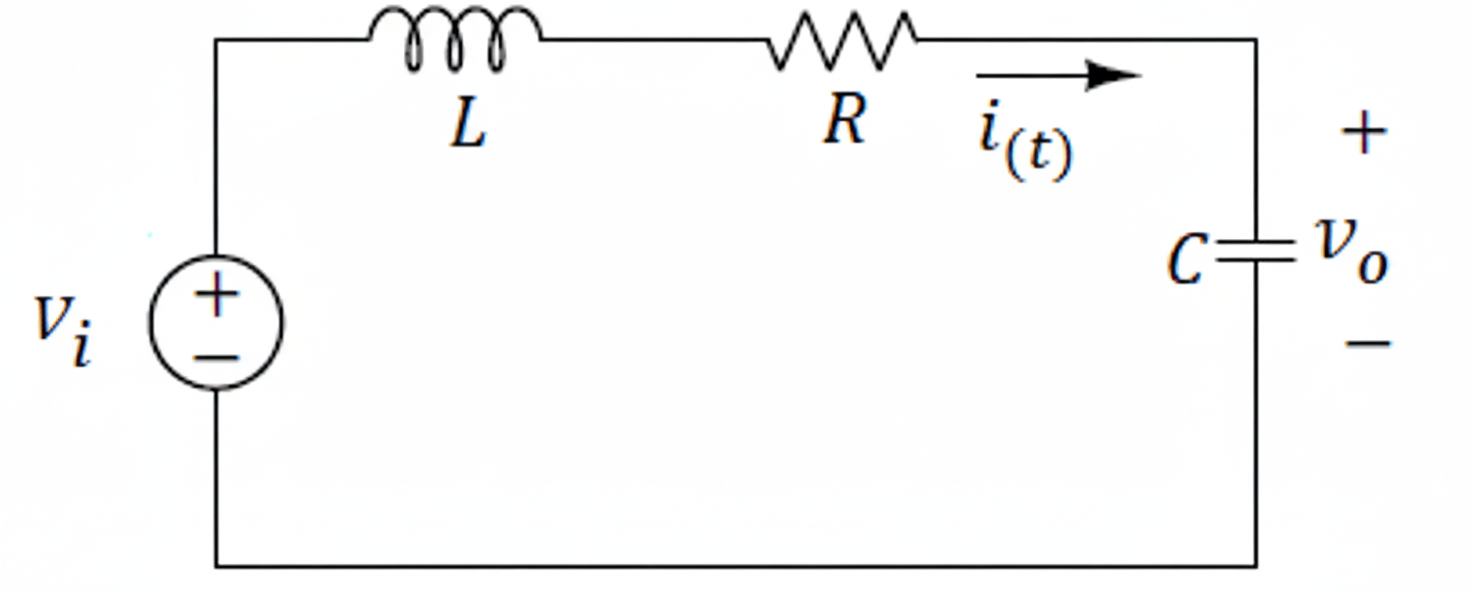
\includegraphics[width=0.4\textwidth]{rlc_serie.png}
        \caption{Circuito RLC en serie}
        \label{fig:rlc_serie}
    \end{figure}

    Determine el valor de \(L\) si \( R_o = 1 k \Omega \) y obtener el valor del capacitor si la nueva frecuencia de la señal de entrada es \(V_i = 20 sen(4000 \pi t)\) usando un escalamiento combinado.

    \textbf{Solución:}
    Primero, calculamos el factor de escalamiento de magnitud \(k_m\):
    \[k_m = \frac{R_o}{R} = \frac{1 k \Omega}{15 k \Omega} = \frac{1}{15} \]
    Luego, calculamos el factor de escalamiento de frecuencia \(k_f\):
    \[k_f = \frac{\omega_o}{\omega_i} = \frac{4000 \pi}{2000 \pi} = 2 \]

    Ahora, usamos \(k_m\) para encontrar el nuevo valor del inductor \(L_o\):
    \[ L_o = k_m \cdot L = \frac{1}{15} \cdot 10 mH = \frac{10}{15} mH = 0.6667 mH \]

    Y con \(k_f\) encontramos el nuevo valor del capacitor \(C_o\):
    \[C_o = C \cdot k_f = 1 \mu F \cdot 2 = 2 \mu F \]

    Por lo tanto, el nuevo valor del inductor es \(L_o = 0.6667 mH\) y el nuevo valor del capacitor es \(C_o = 2 \mu F\).
\end{tcolorbox}

% \section{Bibliografía}
% \renewcommand{\refname}{}
% \begin{thebibliography}{9}
%    \bibitem{} Dr. E. García, \textit{"Diseño Digital VLSI Repaso DDM"}, presentado en el curso de Diseño Digital VLSI, Ciudad de México, 2025.
% \end{thebibliography}

\end{document}
